\documentclass[12pt, a4paper, oneside]{ctexart}
\usepackage{amsmath, amsthm, amssymb, graphicx}
\usepackage{hyperref}
\usepackage{listings}
\usepackage{xcolor}
\usepackage{color}
\usepackage{enumerate}
\usepackage{epstopdf}
\usepackage{float}
\usepackage{framed}
\usepackage[ruled,vlined]{algorithm2e}
\hypersetup{
    colorlinks=true,
    linkcolor=blue,
    filecolor=blue,      
    urlcolor=blue,
    citecolor=cyan,
}
\definecolor{dkgreen}{rgb}{0,0.6,0}
\definecolor{gray}{rgb}{0.5,0.5,0.5}
\definecolor{mauve}{rgb}{0.58,0,0.82}
\definecolor{shadecolor}{rgb}{0.5,0.5,0.5}
\lstset{ %
    language=Python,                % the language of the code
    basicstyle=\footnotesize,           % the size of the fonts that are used for the code
    numbers=left,                   % where to put the line-numbers
    %numberstyle=\tiny\color{gray},  % the style that is used for the line-numbers
    %stepnumber=2,                   % the step between two line-numbers. If it's 1, each line 
                            % will be numbered
    %numbersep=5pt,                  % how far the line-numbers are from the code
    %backgroundcolor=\color{blue},      % choose the background color. You must add \usepackage{color}
    showspaces=false,               % show spaces adding particular underscores
    %showstringspaces=false,         % underline spaces within strings
    showtabs=false,                 % show tabs within strings adding particular underscores
    frame=single,                   % adds a frame around the code
    rulecolor=\color{black},        % if not set, the frame-color may be changed on line-breaks within not-black text (e.g. commens (green here))
    tabsize=2,                      % sets default tabsize to 2 spaces
    captionpos=b,                   % sets the caption-position to bottom
    breaklines=true,                % sets automatic line breaking
    breakatwhitespace=false,        % sets if automatic breaks should only happen at whitespace
    % title=\lstname,                   % show the filename of files included with \lstinputlisting;
                            % also try caption instead of title
    keywordstyle=\color{blue},          % keyword style
    commentstyle=\color{dkgreen},       % comment style
    stringstyle=\color{mauve},         % string literal style
    escapeinside={\%*}{*)},            % if you want to add LaTeX within your code
    morekeywords={*,...}               % if you want to add more keywords to the set
}
\title{ICS\_Lab6\_Report}
\author{Xiaoma}
\date{\today}
\begin{document}
\maketitle
\section*{实验目的}
\begin{itemize}
    \item 使用C/C++复现lab1-4
    \item 考虑到lc-3不支持$*, /, \%, >>, <<$运算,所以只允许使用$ +, -, =, ++, --, ==, !=, <, >, <=, >=, \&, |, ~$
    \item 可以使用\textbf{for , while , do while , if , continue , break , switch case }
\end{itemize}
\section*{实验原理}
\subsection*{lab1}
计算一个16位二进制数a的低b位的个数

依次将a的低b位和1进行与操作,来判断该位是否为1。
\begin{algorithm*}
    \caption{HammingWeight of Lower B Bits}
    \label{alg:algorithm}
    \KwIn{a, b;}
    \KwOut{weight;}
    \BlankLine
    weight = 0;

    judge = 0

    \For{i = 0; i < b; ++i}{
        temp = a \& judge;

        judge += judge;

        \If{temp != 0}{
            ++weight;
        }
    }

    \Return{weight};
\end{algorithm*}
\newpage
\subsection*{lab2}
计算
$$F(0) = F(1) = 1$$
$$F(N) = F(N-2) \% p + F(N-1) \% q \quad (2 \leq N \leq 1024)$$
$$p = 2^{k} \quad (2 \leq k \leq 10),10\leq q \leq 1024$$

采用滑动窗口的方法来求解该问题,\textbf{注意:$F(N-1),F(N-2)$
只有在求和的时候取余,而存储时不需要取余。}
\begin{algorithm*}
    \caption{myFib}
    \label{alg:algorithm}
    \KwIn{p, q, n;}
    \KwOut{F(n);}
    \BlankLine
    num1 = 1

    num2 = 1

    \For{n = n - 1; n > 0; --n}{
        temp1 = (p - 1) \& num1;
        
        temp2 = num2;

        \While{temp2 > 0}{
            temp2 -= q;
        }

        temp2 += q;

        F = temp1 + temp2;
        
        num1 = num2;

        num2 = F;
    }
    \Return{F};
\end{algorithm*}
\newpage
\subsection*{lab3}
实现求字符串的最大重复子串。

通过一次遍历即可求解该问题,记录此时最大重复子串的长度,当出现新的重复子串时,更新最大值。
\begin{algorithm*}
    \caption{maxRepeating}
    \label{alg:algorithm}
    \KwIn{The string : str; Size of str : N;}
    \KwOut{The max-size of repetitive substring : $max\_len$;}
    \BlankLine
    right = str[0];

    left = right;

    max\_len = 1;

    temp = 1;

    \For{i = 1; i < N; ++i}{
        right = str[i];

        i += 1;

        \If(){left == right}{
            temp += 1;
        }
        \Else(){
            \If(){max\_len < temp}{
                max\_len = temp;
            }

            temp = 1;
        }

        left = right;

    }
    \If(){max\_len < temp}{
        max\_len = temp;
    }
    \Return{max\_len};
\end{algorithm*}
\newpage
\subsection*{lab4}
对 16 个人的成绩的升序排列,并求出这 16 个
人中获得评级 A,B 的数量。

为了提高代码效率,在排序的同时计算评级A,B的数量,从而需要获得降序的排名,而题目要求将成绩升序排列,
故如果采用逆序的降序排列,既可以得到正序的升序排列,又可以在排序是计算评级A,B的数量。
\begin{algorithm*}
    \caption{maxRepeating}
    \label{alg:algorithm}
    \KwIn{The scores of students : scores[];}
    \KwOut{The number of A and B: numa, numb;}
    \BlankLine
    numa = 0

    numb = 0

    \For{i = 15; i >= 0; --i}{
        max\_index = i;

        \For{j = i - 1; j >= 0; --j}{
            \If{scores[max\_index] < scores[j]}{
                max\_index = j;
            }
        }

        \If{i != max\_index}{
            swap(scores[max\_index], scores[i]);
        }

        \If(){score[i] >= 85 \& \& num\_a < 4}{
            ++numa;
        }
        \ElseIf(){score[i] >= 85 \& \& num\_a + num\_b < 8}{
            ++numb;
        }
        \ElseIf(){score[i] >= 75 \& \& num\_a + num\_b < 8}{
            ++numb;
        }
    }
    \Return{numa, numb};
\end{algorithm*}

\section*{实验结果}
执行给定的测试用例,结果为
\begin{figure}[H]
    \centering
    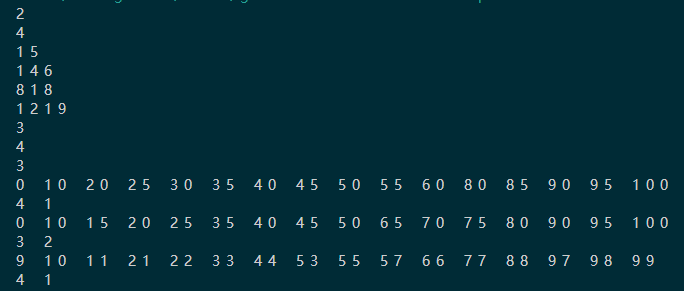
\includegraphics[scale=0.6]{1.png}
\end{figure}
\section*{实验思考}
\begin{itemize}
    \item 高级程序设计语言与lc-3汇编语言编程的区别
    \begin{itemize}
        \item 高级语言可读性、可维护性较佳、代码简洁,lc-3汇编语言的可读性较差、代码繁琐。
        \item lc-3汇编语言程序的占用空间小,执行速度快,执行效率高,高级语言占用的空间大,执行效率较低。
    \end{itemize}
    \item 你认为lc-3汇编语言需要添加哪些指令
    \begin{itemize}
        \item 可以添加取余相关的指令
    \end{itemize}
    \item 对于使用的高级语言,是否需要从lc-3中学到什么
    \begin{itemize}
        \item 通过使用lc-3进行面向寄存器的编程练习,提升了对程序执行时底层原理的理解,可以使我们在后续使用高级语言编程时,更好的提成程序执行效率。
    \end{itemize}
\end{itemize}
\end{document}
